\documentclass[12pt,titlepage]{article}
\usepackage[margin=1.25in]{geometry}
\usepackage{graphicx,amsmath,blindtext,minted}

%% Variables definition
\newcommand{\vSubject}{Islamic Education}
\newcommand{\vSubtitle}{A Summary of Lecture on}
\newcommand{\vSubsubtitle}{Human Beings and Religion}
\newcommand{\vName}{Muhammad Baihaqi Aulia Asy'ari}
\newcommand{\vNIM}{2241720145}
\newcommand{\vClass}{1I}
\newcommand{\vDepartment}{Information Technology}
\newcommand{\vStudyProgram}{D4 Informatics Engineering}

%% [START] Tikz related stuff
\usepackage{tikz}
\usetikzlibrary{svg.path,calc,shapes.geometric,shapes.misc}
\tikzstyle{terminator} = [rectangle, draw, text centered, rounded corners = 1em, minimum height=2em]
\tikzstyle{preparation} = [chamfered rectangle, chamfered rectangle sep=0.75em, draw, text centered, minimum height = 2em]
\tikzstyle{process} = [rectangle, draw, text centered, minimum height=2em]
\tikzstyle{decision} = [diamond, aspect=2, draw, text centered, minimum height=2em]
\tikzstyle{data}=[trapezium, draw, text centered, trapezium left angle=60, trapezium right angle=120, minimum height=2em]
\tikzstyle{connector} = [line width=0.25mm,->]
%% [END] Tikz related stuff

%% [START] Fancy header related stuff
\usepackage{fancyhdr}
\pagestyle{fancy}
\setlength{\headheight}{15pt} % compensate fancyhdr style
\fancyhead{}
\fancyfoot{}
\fancyfoot[L]{\thepage}
\fancyfoot[R]{\textit{\vSubject - \vSubsubtitle}}
\renewcommand{\footrulewidth}{0.4pt}% default is 0pt, overline for footer
%% [END] Fancy header related stuff

%% [START] Custom tabular command related stuff
\usepackage{tabularx}
\newcommand{\details}[2]{
    #1 & #2  \\
}
%% [END] Custom tabular command related stuff

%% [START] Figure related stuff
\newcommand{\image}[3][1]{
    \begin{figure}[h]
        \centering
        \includegraphics[#1]{#2}
        \caption{#3}
        \label{#3}
    \end{figure}
}
%% [END] Figure related stuff

%%
\usepackage{pgf-umlcd}

\renewcommand{\umldrawcolor}{black}
\renewcommand{\umlfillcolor}{white}
%%

%% [BEGIN] Custom enumerator
\usepackage{enumitem}
%% [END] Custom enumerator

%% [START] Arab text
\usepackage{arabtex}
\usepackage{utf8}
\usepackage{unicode}
%% [END] Arab Text

%% [BEGIN] Paragraph indent
\usepackage{indentfirst}
%% [END] Paragraph indent

\begin{document}
\begin{titlepage}
    \centering
    \vfill
    {\bfseries\LARGE
        \vSubject\\
        \vskip0.25cm
        \vSubtitle
        \vskip0.25cm
        \vSubsubtitle
    }
    \vfill
    
\includegraphics[width=6cm]{images/polinema-logo.png}
    \vfill
    {
        \textbf{Name}\\
        \vName\\
        \vskip0.5cm
        \textbf{NIM}\\
        \vNIM\\
        \vskip0.5cm
        \textbf{Class}\\
        \vClass\\
        \vskip0.5cm
        \textbf{Department}\\
        \vDepartment\\
        \vskip0.5cm
        \textbf{Study Program}\\
        \vStudyProgram
    }
\end{titlepage}

\newpage

\textbf{Question: }

\begin{enumerate}
    \item Create class diagram/s for your program design
    \item Create the program that implements class diagram to solve the
    problem of the case above (give comments to give explanation for the
    source code)
    \item Put the (1) class diagram, (2) screenshoot of your program source
    code and (3) screenshoot of the output of the program in a PDF file
    \item Submit the PDF file through your LMS account
\end{enumerate}

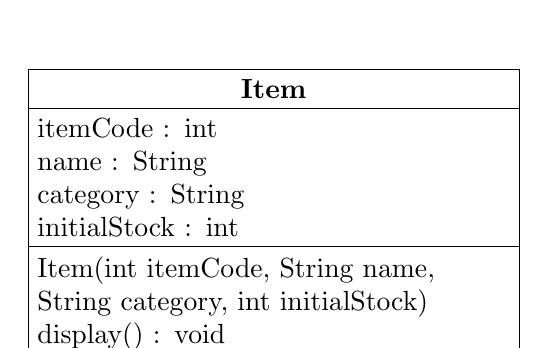
\begin{tikzpicture}
    \begin{class}[text width=6cm]{Item}{0,0}
        \attribute{itemCode : int}
        \attribute{name : String}
        \attribute{category : String}
        \attribute{initialStock : int}
        \operation{Item(int itemCode, String name, String category, int initialStock)}
        \operation{display() : void}
    \end{class}
\end{tikzpicture}
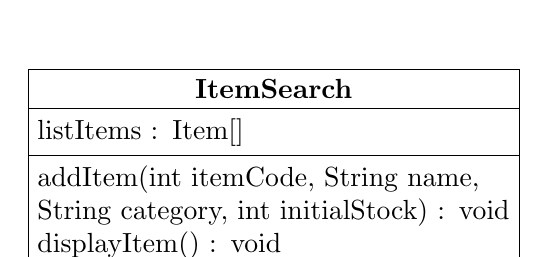
\begin{tikzpicture}
    \begin{class}[text width=6cm]{ItemSearch}{0,0}
        \attribute{listItems : Item[]}
        \operation{addItem(int itemCode, String name, String category, int initialStock) : void}
        \operation{displayItem() : void}
    \end{class}
\end{tikzpicture}
\mbox{}\\
\texttt{Item Class:}
\mbox{}\\
\begin{minted}[autogobble,breaklines,linenos]{java}
    package StockManagement;

    public class Item {
        int itemCode;
        String name;
        String category;
        int initialStock;

        //Item class parametric constructor
        public Item(int itemCode, String name, String category, int initialStock) {
            this.itemCode = itemCode;
            this.name = name;
            this.category = category;
            this.initialStock = initialStock;
        }

        //Display item attributes
        public void display() {
            System.out.printf("Item Code    : %d \n", itemCode);
            System.out.printf("Name         : %s \n", name);
            System.out.printf("Category     : %s \n", category);
            System.out.printf("Initial Stock: %,d\n", initialStock);
        }
    }
\end{minted}
\mbox{}\\
\texttt{ItemSearch Class:}
\mbox{}\\

\begin{minted}[autogobble,breaklines,linenos]{java}
    package StockManagement;

    public class ItemSearch {
        Item[] listItems;

        public ItemSearch(Item[] listItems) {
            this.listItems = listItems;
        }

        /*
        * adding new item in the list
        * creating new list with +1 length and storing every item in that list
        * and then at last appending the new item using the parameter with the item contructor
        */
        public void addItem(int itemCode, String name, String category, int initialStock) {
            Item[] temp = new Item[listItems.length+1];
            for (int i = 0; i < listItems.length; i++) {
                temp[i] = listItems[i];
            }
            temp[temp.length-1] = new Item(itemCode, name, category, initialStock);
            listItems = temp;
        }

        /*
        * displaying all the item by using each item display() function
        */
        public void displayItem() {
            for (Item item : listItems) {
                item.display();
                System.out.println("-------------------------------- --------------------------------");
            }
        }

        public void sortAscendingByInitialStock() {
            Item[] temp = listItems;
            
            for (int i = 0; i < temp.length-1; i++) {
                for (int j = 0; j < temp.length-i; j++) {
                    if (temp[j].initialStock > temp[j-1].initialStock) {
                        /*
                        * swap
                        */
                        Item itemTemp = temp[j];
                        temp[j] = temp[j-1];
                        temp[j-1] = itemTemp;
                    }
                }
            }

            listItems = temp;
        }
        
        public void sortAscendingByItemCode() {
            Item[] temp = listItems;
            
            for (int i = 0; i < temp.length-1; i++) {
                for (int j = 0; j < temp.length-i; j++) {
                    if (temp[j].itemCode > temp[j-1].itemCode) {
                        /*
                        * swap
                        */
                        Item itemTemp = temp[j];
                        temp[j] = temp[j-1];
                        temp[j-1] = itemTemp;
                    }
                }
            }

            listItems = temp;
        }
        
        public void sortAscendingByName() {
            Item[] temp = listItems;
            
            for (int i = 0; i < temp.length-1; i++) {
                for (int j = 0; j < temp.length-i; j++) {
                    if (temp[j].name.charAt(0) > temp[j-1].name.charAt(0)) {
                        /*
                        * swap
                        */
                        Item itemTemp = temp[j];
                        temp[j] = temp[j-1];
                        temp[j-1] = itemTemp;
                    }
                }
            }

            listItems = temp;
        }
        
        public void sortAscendingByCategory() {
            Item[] temp = listItems;
            
            for (int i = 0; i < temp.length-1; i++) {
                for (int j = 0; j < temp.length-i; j++) {
                    if (temp[j].category.charAt(0) > temp[j-1].category.charAt(0)) {
                        /*
                        * swap
                        */
                        Item itemTemp = temp[j];
                        temp[j] = temp[j-1];
                        temp[j-1] = itemTemp;
                    }
                }
            }

            listItems = temp;
        }


    }
\end{minted}

\mbox{}\\
\texttt{ItemMain Class:}
\mbox{}\\

\begin{minted}[autogobble,breaklines,linenos]{java}
    package StockManagement;

    public class ItemMain {
        public static void main(String[] args) {
            Item[] listItems = new Item[9];
            listItems[0] = new Item(16030927, "Indomilk", "drink", 100);
            listItems[1] = new Item(16100617, "Sprite", "drink", 70);
            listItems[2] = new Item(16240401, "Yakult", "drink", 500);
            listItems[3] = new Item(16270525, "Indomie", "food", 250);
            listItems[4] = new Item(16971204, "Oreo", "food", 320);
            listItems[5] = new Item(16100727, "Chocochips", "food", 120);
            listItems[6] = new Item(16460329, "Ballpoint", "stationary", 75);
            listItems[7] = new Item(16320421, "Pencil", "stationary", 110);
            listItems[8] = new Item(16180729, "Book", "stationary", 57);
            ItemSearch itemSearch = new ItemSearch(listItems);
        }
    }
\end{minted}

\end{document}